\documentclass[11pt]{article}

\usepackage{graphicx}
\usepackage{wrapfig}
\usepackage{url}
\usepackage{wrapfig}
\usepackage{color}
\usepackage{marvosym}
\usepackage{enumerate}
\usepackage{subfigure}
\usepackage{tikz}
\usepackage{amsmath}
\usepackage{amssymb}
\usepackage{hyperref}
\usepackage{bbm}


\oddsidemargin 0mm
\evensidemargin 5mm
\topmargin -20mm
\textheight 240mm
\textwidth 160mm



\newcommand{\vwi}{{\bf w}_i}
\newcommand{\vw}{{\bf w}}
\newcommand{\vx}{{\bf x}}
\newcommand{\vy}{{\bf y}}
\newcommand{\vxi}{{\bf x}_i}
\newcommand{\yi}{y_i}
\newcommand{\vxj}{{\bf x}_j}
\newcommand{\vxn}{{\bf x}_n}
\newcommand{\yj}{y_j}
\newcommand{\ai}{\alpha_i}
\newcommand{\aj}{\alpha_j}
\newcommand{\X}{{\bf X}}
\newcommand{\Y}{{\bf Y}}
\newcommand{\vz}{{\bf z}}
\newcommand{\code}[1]{{\footnotesize \tt #1}}
\newcommand{\ztnodesize}{.6}

\pagestyle{myheadings}
\markboth{Homework 5}{Spring 2018 CS 475 Machine Learning: Homework 5}


\title{CS 475 Machine Learning: Homework 5\\Probabilistic Graphical Models\\
	\Large{Due: Friday May 4, 2018, 11:59pm}\\
	75 Points Total \hspace{1cm} Version 1.0}
\author{}
\date{}

\begin{document}
	\large
	\maketitle
	\thispagestyle{headings}
	
	\vspace{-.5in}
	
	{\bf Make sure to read from start to finish before beginning the assignment.}
\section{Programming (60 points)}

In this assignment you will implement the sum-product algorithm for calculating marginal probabilities, as well as the max-sum algorithm for finding the configuration that gives the highest global probability in a linear chain MRF (more specifically, a factor graph). You will implement sum-product and max-sum on top of the potential functions that we give you. There is no learning in this homework, only exact inference.

\subsection{The Factor Graph} %%%%%%%%%%%%%%%%%%%%%%%%%%%%%%%%%%%%%%%%%%%%%%%%%%%%%%%%%%%%%
\newcommand{\factorsize}{1}
\newcommand{\nodesize}{1.3}
\begin{figure}[h]
	\begin{center}
\begin{tikzpicture}[style=thick,scale=1]
			\begin{scope}[shape=circle,minimum size=0.1cm]
			\tikzstyle{every node}=[draw,fill]
			\node[fill=red,scale= \factorsize,shape=rectangle] (F_1) at (0,1.5) {$\mathbf{f_{1}}$};
			\node[fill=none,scale=\nodesize] (X_1) at (0,0) {$\mathbf{X_1}$};
			\node[fill=red,scale= \factorsize,shape=rectangle] (F_N1) at (2,0) {$\mathbf{f_{n+1}}$};
			\node[fill=red,scale= \factorsize,shape=rectangle] (F_2) at (4,1.5) {$\mathbf{f_{2}}$};
			\node[fill=none,scale=\nodesize] (X_2) at (4,0) {$\mathbf{X_2}$};
			\node[fill=red,scale= \factorsize,shape=rectangle] (F_N2) at (6,0) {$\mathbf{f_{n+2}}$};
			\node[fill=red,scale= \factorsize,shape=rectangle] (F_3) at (8,1.5) {$\mathbf{f_{\ldots}}$};
			\node[fill=none,scale=\nodesize] (X_3) at (8,0) {$\mathbf{...}$};
			\node[fill=red,scale= \factorsize,shape=rectangle] (F_N3) at (10,0) {$\mathbf{f_{2n-1}}$};
			\node[fill=red,scale= \factorsize,shape=rectangle] (F_4) at (12,1.5) {$\mathbf{f_{n}}$};
			\node[fill=none,scale=\nodesize] (X_4) at (12,0) {$\mathbf{X_n}$};
			\draw [-] (X_1) -- (F_1);
			\draw [-] (X_2) -- (F_2);
			\draw [-] (X_3) -- (F_3);
			\draw [-] (X_4) -- (F_4);
			\draw [-] (X_1) -- (F_N1);
			\draw [-] (F_N1) -- (X_2);
			\draw [-] (X_2) -- (F_N2);
			\draw [-] (F_N2) -- (X_3);
			\draw [-] (X_3) -- (F_N3);
			\draw [-] (F_N3) -- (X_4);
			\end{scope}
		\end{tikzpicture}
		\caption{The factor graph that will be used in this assignment}
			\label{fig:factor_graph}
		\end{center}
\end{figure}
Each of the variables in our chain (the $x_i$) are $k$-ary discrete variables.


\subsection{Sum-product Algorithm} %%%%%%%%%%%%%%%%%%%%%%%%%%%%%%%%%%%%%%%%%%%%%%%%%%%%%%%%
There are several presentations of the sum-product algorithm. We will follow the presentation in class, which is based on section 8.4.4 of Bishop. For more details and diagrams, you can see this chapter (which is available freely online \href{https://www.microsoft.com/en-us/research/wp-content/uploads/2016/05/Bishop-PRML-sample.pdf}{https://www.microsoft.com/en-us/research/wp-content/uploads/2016/05/Bishop-PRML-sample.pdf}).

Our goal is to find the marginal probability of a node in our factor graph.  Applying the sum-product algorithm and leveraging the linear structure of the graph, we write this marginal probability as:
\begin{equation}
\label{eq:sum-product}
	p(x) = \prod_{s \in N(x)} \Bigg[ \sum_{X_s} F_s(x, X_s) \Bigg]
\end{equation}
where:\\
\indent $N(x)$ is the set of all factor node neighbors of $x$\\
\indent $F_s(x, X_s)$ represents the product of all the factors ``downstream" of $f_s$\\
\\
Part of the above equation will be used many times, so for the sake of computation and intuition we will define the sum term as a ``message" $\mu$:
\begin{equation}
\label{eq:f2x}
	\mu_{f_s \rightarrow x}(x) := \sum_{X_s} F_s(x, X_s)
\end{equation}
If you look at the diagram in the book, you will see the recursive nature of $F_s(x, X_s)=f_s(x,x_1,\ldots,x_M) \prod\limits_{m \in N(f_s) \setminus x} \mu_{x_m \rightarrow f_s(x_m)}$, where $X_s=\{x_m|m \in N(f_s) \setminus x\}$. Our base case is:
\[
	\mu_{f \rightarrow x}(x) := f(x) \text{ iff the only neighbor of f is x}
\]
\\
The sum-product algorithm defines the message from a variable node to a factor node as the product of the messages it receives from its ``downstream" factors:
\begin{equation}
	\mu_{x \rightarrow f_s} := \prod_{l \in N(x) \setminus s} \mu_{f_l \rightarrow x}(x)
\end{equation}
\\
As before, there is a base case for this equation:
\[
	\mu_{x \rightarrow f}(x) := 1 \text{ iff the only neighbor of x is f}
\]
\\
And we're done: we can find marginal probabilities using equation 1. While seemingly simple, the details may be a bit opaque. To help clarify them, you will implement sum-product on the linear chain factor graph above.

\subsection{Max-sum Algorithm} %%%%%%%%%%%%%%%%%%%%%%%%%%%%%%%%%%%%%%%%%%%%%%%%%%%%%%%%
Instead of finding a marginal probability of a set of variables taking some values, in this task our goal is to find a setting of the variables that has the maximal probability. We can find this configuration and the associated probability using the ``Max-Sum Algorithm''. Conceptually, the main difference between sum-product and max-sum is that, while sum-product finds the distribution over a set of variables, of which the max is \textit{locally} most likely, max-sum finds the configuration that is globally most likely, i.e., maximizes the joint distribution:
\begin{equation}
    x^{max} = \arg\max\limits_x p(x)
\end{equation}
The value of the corresponding probability is given by:
\begin{equation}
    p(x^{max}) = \max\limits_x p(x)
\end{equation}
The message passing scheme in max-sum is similar to that in sum-product. We only need to replace the ``marginalization'' with ``maximization'' in Eq.~(\ref{eq:sum-product}) and (\ref{eq:f2x}) as:
\begin{equation}
	p(x) = \prod_{s \in N(x)} \Bigg[ \max_{X_s} F_s(x, X_s) \Bigg]
\end{equation}

\begin{equation}
    \mu_{f_s \rightarrow x}(x) := \max_{X_s} F_s(x, X_s)
\end{equation}
The joint probability $p(x)$ is usually quite small, which might lead to inaccuracy of the computation due to the underflow problem. Therefore in practice we take the logarithm of probability values and push ``log'' into all terms so that all the products of probabilities are now replaced with sums of logarithm of probabilities. That is why the algorithm is called ``Max-Sum''. You might see ``Max-Product'' which refers to the same algorithm. The distinction refers
to whether or not you use $\log$s.

In order to recover the configuration of all variables (i.e., the value for each variable) after the largest joint probability is found, we also need to record the assignment $\arg\max_{X_s} F_s(x, X_s)$ for $X_s$ along with the message $\mu_{f_s \rightarrow x}(x)$, which means that $X_s$ is configured as $\arg\max_{X_s} F_s(x, X_s)$ if $x$ is configured as some value. Consequently, at the moment the largest joint probability is computed, we can backtrack to obtain values for each variable.

Putting everything together, the goal is to compute:
\begin{eqnarray}
\max\limits_x p(x) &=& \max_x \sum_{s \in N(x)} \Bigg[ \mu_{f_s \rightarrow x}(x) \Bigg] \\
\mu_{f_s \rightarrow x}(x) &:=& \left\{ \begin{array}{ll}
                                    \log f_s(x) & \text{ if the only neighbor of $f_s$ is $x$} \\
                                    \max\limits_{x_1,\ldots,x_M} \Bigg[ \log f_s(x,x_1,\ldots,x_M) + \sum\limits_{m \in N(f_s) \setminus x} \mu_{x_m \rightarrow f_s(x_m)} \Bigg] & \text{otherwise}
                                          \end{array} \right. \\
\mu_{x \rightarrow f_s}(x) &:=& \left\{ \begin{array}{ll}
                                    0 & \text{ if the only neighbor of $x$ is $f_s$} \\
                                    \sum\limits_{l \in N(x) \setminus s} \mu_{f_l \rightarrow x}(x) & \text{otherwise}
                                          \end{array} \right.
\end{eqnarray}
where $X_s=\{x_m|m \in N(f_s) \setminus x\}$ is recorded for $x$ along with the message $\mu_{f_s \rightarrow x}(x)$.

You can find details on this algorithm in section 8.4.5 of Bishop.

\subsection{Implementation} %%%%%%%%%%%%%%%%%%%%%%%%%%%%%%%%%%%%%%%%%%%%%%%%%%%%%%%%%%%%%%

For the factor graph in this assignment, there are unary ($f_1$ to $f_n$) and binary ($f_{n+1}$ to $f_{2n-1}$) factors, and each factor $f_i$ is associated with a potential function $\psi_i$.
Each unary factor will have a potential function $\psi_{i}(a)$ which returns a real non-negative value corresponding to the potential when variable $x_{i}$ takes value $a$. Each factor node between two variable nodes will have a potential function $\psi_{i}(a, b)$ which returns a value corresponding to the potential when variable $x_{i-n}$ takes value $a$ and node $x_{i-n+1}$ takes value $b$. Recall that every $x_i$ can take values from $1$ to $k$.\\
\\
We will provide you code that gives you values of $\psi_i(a)$ and $\psi_i(a, b)$. They will be in the class \code{chain\_mrf.ChainMRFPotentials} and have the signatures:
\begin{verbatim}
    potential(self, i, a)
    potential(self, i, a, b)
\end{verbatim}
There are $n$ nodes in this chain, so the value of \code{i} must be between 1 and $n$ (inclusive) in the first method and between $n+1$ and $2n-1$ (inclusive) in the second method. Since every $x_i$ can take values from 1 to $k$ (inclusive), you must only call this function with values for \code{a} and \code{b} between 1 and $k$ (inclusive). You will be able to get values for $n$ and $k$ by calling the following functions in \code{chain\_mrf.ChainMRFPotentials}:
\begin{verbatim}
    chain_length(self)  // returns n
    num_x_values(self)   // returns k
\end{verbatim}
These values will be read into \code{chain\_mrf.ChainMRFPotentials} from a text file that must be provided in the constructor:
\begin{verbatim}
    __init__(self, data_file)
\end{verbatim}
We are providing you with a sample of this data file, \code{sample\_mrf\_potentials.txt}. The format is \code{"n k"} on the first line and either \code{"i a potential"} or \code{"i a b potential"} on subsequent lines. Feel free to try out new chains to get different probability distributions, just make sure it contains all the needed potential values.

Since our graph is a chain, which means that the number of elements in $X_s=\{x_m|m \in N(f_s) \setminus x\}$ is at most 1, we can simply create a 1D array of length $k$ for each variable $x$ for backtracking. \textbf{In case of a tie, always choose the lowest value of a variable}.

Your code will work by calculating these messages given the value of the potential functions between the variable nodes in the chain. For details on how to do this, you can refer to your notes from class or see Bishop's examples in the book.


\subsection{What You Need to Implement} %%%%%%%%%%%%%%%%%%%%%%%%%%%%%%%%%%%%%%%%%%%%%%%%%%%%
We have provided you with two classes, \code{chain\_mrf.SumProduct} and \code{chain\_mrf.MaxSum}, with one method for each left blank that you will need to implement:
\begin{verbatim}
class SumProduct:
    def marginal_probability(self, x_i):
        // TODO

class MaxSum:
    def max_probability(self, x_i):
        // TODO
\end{verbatim}
 The first should return a \textbf{python list of type float} where the $j$-th element is the probability that $x_i = j$. The length of this list should be $\mathbf{k+1}$ and you should leave the 0 index as 0. These are probabilities so don't forget to normalize to sum to 1.

 The second should return a \textbf{float scalar} which is the logarithm of the joint probability corresponding to the most probable setting of all variables. The assignment of each variable should be stored in the class member variable \code{\_assignments}, which is a \textbf{python list of type int} of length $\mathbf{n+1}$. Note that different values for \code{x\_i} of the method \code{max\_probability} should give the same result. You should use \code{math.log} for logarithm computations.


\subsection{How We Will Run Your Code} %%%%%%%%%%%%%%%%%%%%%%%%%%%%%%%%%%%%%%%%%%%%%%%%%%%%
We will run your code by providing you with a single command line argument, which is the data file:
\begin{verbatim}
    python chain_mrf_tester.py mrf_potentials.txt
\end{verbatim}
Note that we will use new data files with different values of $n$ and $k$, so make sure your code works for any reasonable input.\\
\\
Your output should just be the results of the print statements in the code given. {\bf Do not print anything else in the version you hand in.}
	
\section{Analytical (15 points)}
	
\paragraph{1) (15 points)} The probability density function of most Markov Random Fields cannot be factorized as the product of a few conditional probabilities. This question explores some MRFs that can be factorized in this way.

Consider the graph structure in Figure \ref{fig:utm1}.
\begin{figure}[h]
	\begin{center}
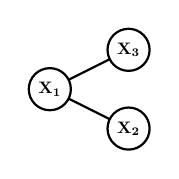
\begin{tikzpicture}[style=thick,scale=1] 
			\begin{scope}[shape=circle,minimum size=0.1cm] 
			\tikzstyle{every node}=[draw,fill] 
			\node[fill=none,scale=\ztnodesize] (X_1) at (0,0.5) {$\mathbf{X_1}$};
			\node[fill=none,scale=\ztnodesize] (X_2) at (1,0) {$\mathbf{X_2}$};
			\node[fill=none,scale=\ztnodesize] (X_3) at (1,1) {$\mathbf{X_3}$};
			\draw [-] (X_1) -- (X_2);
			\draw [-] (X_1) -- (X_3);
			\end{scope} 
		\end{tikzpicture}
		\caption{The Original Undirected Graph}
			\label{fig:utm1}
		\end{center}
\end{figure}
From this graph, we know that $X_2$ and $X_3$ are conditionally independent given $X_1$. We can draw the corresponding directed graph as Figure \ref{fig:dtm2}.
\begin{figure}[h]
	\begin{center}
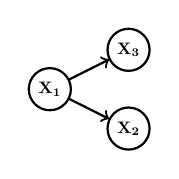
\begin{tikzpicture}[style=thick,scale=1] 
			\begin{scope}[shape=circle,minimum size=0.1cm] 
			\tikzstyle{every node}=[draw,fill] 
			\node[fill=none,scale=\ztnodesize] (X_1) at (0,0.5) {$\mathbf{X_1}$};
			\node[fill=none,scale=\ztnodesize] (X_2) at (1,0) {$\mathbf{X_2}$};
			\node[fill=none,scale=\ztnodesize] (X_3) at (1,1) {$\mathbf{X_3}$};
			\draw [->] (X_1) -- (X_2);
			\draw [->] (X_1) -- (X_3);
			\end{scope} 
		\end{tikzpicture}
		\caption{The Converted Directed Graph}
			\label{fig:dtm2}
		\end{center}
\end{figure}
This suggests the following factorization of the joint probability:
\begin{eqnarray}
P(X_1, X_2, X_3) = P(X_3 | X_1) P(X_2 | X_1) P(X_1) \nonumber
\end{eqnarray}

Now consider the following graphical model in Figure \ref{fig:utm}.
\begin{figure}[h!]
	\begin{center}
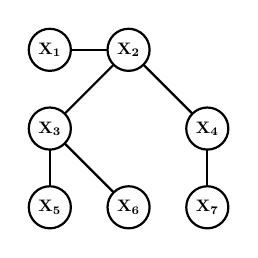
\begin{tikzpicture}[style=thick,scale=1] 
			\begin{scope}[shape=circle,minimum size=0.1cm] 
			\tikzstyle{every node}=[draw,fill] 
			\node[fill=none,scale=\ztnodesize] (X_1) at (0,2) {$\mathbf{X_1}$};
			\node[fill=none,scale=\ztnodesize] (X_2) at (1,2) {$\mathbf{X_2}$};
			\node[fill=none,scale=\ztnodesize] (X_3) at (0,1) {$\mathbf{X_3}$};
			\node[fill=none,scale=\ztnodesize] (X_4) at (2,1) {$\mathbf{X_4}$};
			\node[fill=none,scale=\ztnodesize] (X_5) at (0,0) {$\mathbf{X_5}$};
			\node[fill=none,scale=\ztnodesize] (X_6) at (1,0) {$\mathbf{X_6}$};
			\node[fill=none,scale=\ztnodesize] (X_7) at (2,0) {$\mathbf{X_7}$};
			\draw [-] (X_1) -- (X_2);
			\draw [-] (X_2) -- (X_3);
			\draw [-] (X_2) -- (X_4);
			\draw [-] (X_3) -- (X_5);
			\draw [-] (X_3) -- (X_6);
			\draw [-] (X_4) -- (X_7);
			\end{scope} 
		\end{tikzpicture}
		\caption{An Undirected Graph}
			\label{fig:utm}
		\end{center}
\end{figure}

As before, we can read the conditional independence relations from the graph. 
\begin{enumerate}[(a)]
\item Following the example above, write a factorization of the joint distribution:

\begin{center}
$P(X_1,X_2,X_3,X_4,X_5,X_6,X_7)$.
\end{center}

\item Is this factorization unique, meaning, could you have written other factorizations that correspond this model? If the factorization is unique, explain why it is unique. If it is not unique, provide an alternate factorization.
\item What is it about these examples that allows them to be factored in this way? Show an example MRF that cannot be factored in this way.
\end{enumerate}
	
\section{What to Submit}
	You will need to create an account on gradescope.com and signup for this class. The course is \href{https://gradescope.com/courses/13142}{\url{https://gradescope.com/courses/13142}}. Use entry code {\tt 974Z3W}. See this video for instructions on how to upload a homework assignment: \href{https://www.youtube.com/watch?v=KMPoby5g_nE}{\url{https://www.youtube.com/watch?v=KMPoby5g_nE}}. In each assignment you will submit two things to gradescope.
	\begin{enumerate}
		\item \textbf{Submit your code (.py files) to gradescope.com as a zip file}. \textbf{Your code must be uploaded as code.zip with your code in the root directory}. By `in the root directory,' we mean that the zip should contain \texttt{*.py} at the root (\texttt{./*.py}) and not in any sort of substructure (for example \texttt{hw4/*.py}). One simple way to achieve this is to zip using the command line, where you include files directly (e.g., \texttt{*.py}) rather than specifying a folder (e.g., \texttt{hw4}):
		\begin{verbatim}
		zip code.zip *.py
		\end{verbatim}
		
		We will run your code using the exact command lines described earlier, so make sure it works ahead of time, and make sure that it doesn't crash when you run it on the test data. Remember to submit all of the source code, including what we have provided to you. We will include {\tt requirements.txt} but nothing else.
		\item \textbf{Submit your writeup to gradescope.com}. \textbf{Your writeup must be compiled from latex and uploaded as a PDF}. It should contain all of the answers to the analytical questions asked in the assignment. Make sure to include your name in the writeup PDF and to use the provided latex template for your answers. 
	\end{enumerate}
	
	\section{Questions?}
	Remember to submit questions about the assignment to the appropriate group on Piazza: \href{https://piazza.com/class/jatranyaky957s}{\url{https://piazza.com/class/jatranyaky957s}}.
	
\end{document}